\section{Binomial distributed values}
In the following subsections the performance of the different algorithms is tested for different kinds of inputs.
The exact distributions of the input are explained separately in each subsection.
The procedure for each comparison is always the same. A random input is generated according to the distribution and then solved by every algorithm.
All algorithms had the same two stopping conditions.
The first was reaching a perfect partition and the second was taking more than $100 \cdot n\ln(n)$ steps or $10 \cdot n\ln(n)$ in some cases.
For the lower values of $n$ the step limit of 100,000 was used instead.
For $n=20$ giving the algorithm only 600 steps is rather small.
In some cases the smaller inputs are even more difficult to solve.
Most modern computer should be able to handle 100,000 iterations in a short amount of time anyway.
So the minimum step limit of 100,000 seemed reasonable.
If either of these conditions was met, the algorithm returned its current best solution.
This step is repeated 1000 times.
The results are presented in a table containing multiple statistics for each algorithm over all 1000 runs.
The data is explained in the table below.

\begin{tabular}{c|l}
      column name     & meaning                                                         \\ \hline
      algo type       & type of algorithm (RLS, RLS-N, RLS-R, (1+1)EA or pmut)          \\
      algo param      & parameter of the algorithm or '-' if it is the standard variant \\
      avg mut/change  & average \#bits flipped for iterations leading to an improvement \\
      avg mut/step    & average \#bits flipped for any iteration                        \\ \hline
      total avg count & average \#iterations for all runs                               \\
      avg eval count  & average \#iterations of runs returning an optimal solution      \\
      max eval count  & maximum \#iterations of runs returning an optimal solution      \\
      min eval count  & minimum \#iterations of runs returning an optimal solution      \\ \hline
      fails           & number of runs that did not find an optimal solution            \\
      fail ratio      & ratio of unsuccessful runs to all runs                          \\
      avg fail dif    & average value of $b_F-f(opt)$ for non-optimal solutions         \\
\end{tabular}

Firstly the different variants of the RLS are compared with values of $k \in\{2,3,4\}$, then the performance of the (1+1) EA with static mutation rate $c/n$ with $c \in\{1,2,3,5,10,50,100\}$ and lastly the performance of the $pmut_\beta$ mutation operator with the parameter $\beta \in \{-1.25, -1.5, \dots, -2.75,-3.0,-3.25\}$.
Additionally the best variants of each algorithm are compared in another 1000 runs.
Afterwards there is also a comparison for multiple input sizes of the best algorithms because the best algorithm is often dependent on the size of the input.
Normally there are three tables for each input.
The first states how often the algorithms did not find an optimal solution for the different input sizes ('fails' in top left cell).
The second gives their average performance for the successful runs ('avg' in top left cell) and the last the performance for all runs ('total avg' in top left cell).
The last two tables differ in the unsuccessful runs. Often the algorithm is stuck in a local optima it won't leave in reasonable time or never for variants of the RLS.
In these cases the step limit is the deciding factor on how big the penality for this run is.
So neither of the two average values alone is enough to give a complete insight on the performance.
Sometimes a variant of the RLS is much faster than the other algorithms for a specific input but is also the only algorithm to get stuck in a local optimum.
This creates the possibility to start the RLS variant with a low step limit and switch to the (1+1) EA if the RLS variant does not return an optimal solution.
Giving both tables for the different average values might help with this decision.

The first analysed inputs are inputs following a binomial distribution \textasciitilde$B(m,p)$ as those inputs have been researched in the previous subsection.
The results showed that the expected value of a single number is the main driver for the amount of perfect partitions the input has.
The results also suggested the inputs tend to have more perfect partitions if the expected value is lower.
The more perfect partitions an input has relative to the number of all possible partitions, the more likely the different RSHs are to find one of those.
Therefore researching inputs with higher expected values seems more interesting but generating higher values takes more time with a random number generator that needs $\mathcal{O}(mp)$ time.
To keep the time for generating one set of numbers reasonable the values chosen for all tests are $m=10000, p=0.1, n=10000$ with the expected value for a single number being $mp=1000$.
Figure~\ref{fig:binDistExample} shows a random binomial distributed input of length $n=10000$.
All elements are sharply concentrated around the expected value with all values being at $1000\pm200$.
So after reaching a difference between the two bins of below $(1000-200)/2=400$ the algorithm can no longer achieve an improvement by flipping a single bit.

\begin{figure}[h]
      \caption{Distribution of a random binomial input}
      \centering
      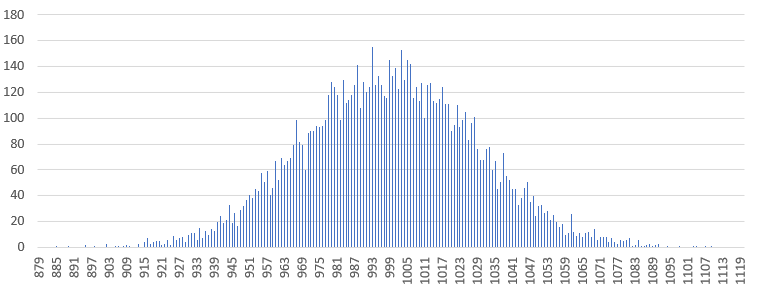
\includegraphics[width=0.7\textwidth]{figures/images/numberGenerator/binomialDistributionForN10000p0_1.png}\label{fig:binDistExample}
\end{figure}
\subsection{RLS Comparison}


\makebox[\linewidth]{
\begin{tabular}{lp{3cm}p{6cm}p{6cm}}
\begin{tabular}[h]{cccccccc}
algo type&            \RLSN&     \RLSR&     \RLSR&     \RLSN&     \RLSR&     \RLSN&       RLS\\
algo param&             b=2&       s=3&       s=4&       b=3&       s=2&       b=4&         -\\
avg mut/change&       2.000&     1.996&     2.476&     3.000&     1.502&     4.000&     1.000\\
avg mut/step&         2.000&     2.000&     2.500&     3.000&     1.500&     4.000&     1.000\\
\hline
total avg count&     83,118&   104,748&   105,513&   112,223&   114,486&   121,927& 2,443,567\\
avg eval count&      83,118&   104,748&   105,513&   112,223&   114,486&   121,927&    45,834\\
max eval count&     778,110& 1,453,252&   898,974& 1,377,471&   915,268&   816,633&   485,275\\
min eval count&         197&       126&        45&       212&       271&       155&       128\\
\hline
fail ratio&           0.000&     0.000&     0.000&     0.000&     0.000&     0.000&     0.447\\
avg fail dif&             -&         -&         -&         -&         -&         -&         1\\
\end{tabular}
\end{tabular}
}


The $\text{RLS-N}_2$ seems to perform the best as it mostly switches two elements which works great for binomial distributed inputs. 
The same algorithm with $k=4$ performs a bit worse but still good as switching 4 elements can be beneficial as well.
The variant of RLS-N with $k=3$ on the other hand does not reach the optimal solution in 23.4\% of the inputs with an average difference of 1.
It also needs 1000 times more iterations to find the optimal on average compared to the best algorithm RLS-N$_2$.
The RLS-R variants behave mostly the same with $k=2$ being the best, followed by $k=4$ and $k=3$.
In this case the variant of $k=3$ is by far not as bad as for the RLS-N$_3$ because the probability of flipping 2 bits is 1/3 as compared to $\mathcal{O}(n^{-1})$ for the RLS-N$_3$.
The RLS-R seem all to be a good option for binomial inputs with values of $k\in\{2,3,4\}$.
The standard RLS on the other hand performs by far the worst as it only moves one element per step.
It only managed to reach the optimal solution once for 1000 different inputs.
The number of iterations for this input was only 50 so the RLS likely had a good initialisation with a few lucky steps leading directly to the optimum.
For all other cases the average difference between the bins was 254 which is close to the median of the values from 0 to $(1000-100)/2=450$.
This is likely due to the RLS being unable to improve the solution once the current solution has a difference below half of the lowest value (Corollary~\ref{cor:RLSStuck}).
\subsection{(1+1) EA Comparison}
For the (1+1) EA the best static mutation rate seems to be $3/n$. 
The probability of flipping 2 or 4 bits as n goes to infinity for mutation rate $1/n$ approaches $13/24e\approx 0.199$, for $2/n$ approaches $8/3e^2\approx 0.361$, for $3/n$ approaches $63/8e^3\approx 0.392$, for $4/n$ approaches $56/3e^4\approx 0.342$ and for $5/n$ approaches $77/2e^5\approx 0.259$.
So the highest probability has $c=3$, followed by $c=4$ and $c=2$ then $c=5$ and lastly $c=1$.
For higher values of $c$ the probability decreases further as the expected number of flipped bits is $c$ for mutation rate $c/n$.

\makebox[\linewidth]{
\begin{tabular}{lp{3cm}p{6cm}p{6cm}}
\begin{tabular}[h]{ccccccccc}
algo type&          (1+1) EA&   (1+1) EA&   (1+1) EA&   (1+1) EA&      (1+1) EA&   (1+1) EA&   (1+1) EA&   (1+1) EA\\
algo param&           3/n&     4/n&     2/n&     5/n&       -&    10/n&    50/n&   100/n\\
avg mut/change&     3.101&   3.968&   2.343&   4.859&   1.698&   9.732&  49.544&  99.494\\
avg mut/step&       2.999&   4.003&   2.002&   4.999&   1.001&   9.998&  49.998&  99.997\\
\hline
total avg count&      646&     701&     706&     857&   1,123&   1,508&   8,175&  15,485\\
avg eval count&       646&     701&     706&     857&   1,123&   1,508&   8,175&  15,485\\
max eval count&     5,346&   5,692&   3,415&   5,572&   7,001&  12,112&  52,831& 145,269\\
min eval count&        23&       4&      30&       9&      23&      14&      27&      69\\
\hline
fails&                  0&       0&       0&       0&       0&       0&       0&       0\\
fail ratio&         0.000&   0.000&   0.000&   0.000&   0.000&   0.000&   0.000&   0.000\\
avg fail dif&           -&       -&       -&       -&       -&       -&       -&       -\\
\end{tabular}
\end{tabular}
}


The static mutation rate $3/n$ seems to perform the best with both $4/n$ and $2/n$ being a close second place.
The next best values are $5/n$ and the standard $1/n$ both having a clear difference between each other and the better parameters.
From then on the number of iterations rises monotonically with rising mutation rate.
The higher mutation rates perform significantly worse but the still find a solution within the limit as opposed to the standard RLS.
\subsection{pmut Comparison}


\makebox[\linewidth]{
\scriptsize
\begin{tabular}{lp{3cm}p{6cm}p{6cm}}
\begin{tabular}[h]{m{2.5cm}m{0,40cm}m{0,40cm}m{0,40cm}m{0,40cm}m{0,40cm}m{0,40cm}m{0,40cm}m{0,40cm}m{0,40cm}m{0,40cm}m{0,40cm}m{0,40cm}m{0,40cm}m{0,40cm}m{0,40cm}m{0,40cm}m{0,40cm}m{0,40cm}}
\multicolumn{1}{c}{algo type}&\multicolumn{2}{c}{            pmut}&\multicolumn{2}{c}{     pmut}&\multicolumn{2}{c}{     pmut}&\multicolumn{2}{c}{     pmut}&\multicolumn{2}{c}{     pmut}&\multicolumn{2}{c}{     pmut}&\multicolumn{2}{c}{     pmut}&\multicolumn{2}{c}{     pmut}&\multicolumn{2}{c}{     pmut}\\
\multicolumn{1}{c}{algo param}&\multicolumn{2}{c}{           3.25}&\multicolumn{2}{c}{     3.00}&\multicolumn{2}{c}{     2.75}&\multicolumn{2}{c}{     2.50}&\multicolumn{2}{c}{     2.25}&\multicolumn{2}{c}{     2.00}&\multicolumn{2}{c}{     1.75}&\multicolumn{2}{c}{     1.50}&\multicolumn{2}{c}{     1.25}\\
\multicolumn{1}{c}{avg mut/change}&\multicolumn{2}{c}{      1.583}&\multicolumn{2}{c}{    1.737}&\multicolumn{2}{c}{    2.002}&\multicolumn{2}{c}{    2.423}&\multicolumn{2}{c}{    3.303}&\multicolumn{2}{c}{    5.830}&\multicolumn{2}{c}{   12.519}&\multicolumn{2}{c}{   30.910}&\multicolumn{2}{c}{   73.182}\\
\multicolumn{1}{c}{avg mut/step}&\multicolumn{2}{c}{        1.729}&\multicolumn{2}{c}{    1.934}&\multicolumn{2}{c}{    2.274}&\multicolumn{2}{c}{    2.895}&\multicolumn{2}{c}{    4.360}&\multicolumn{2}{c}{    8.452}&\multicolumn{2}{c}{   22.278}&\multicolumn{2}{c}{   70.532}&\multicolumn{2}{c}{  224.421}\\
\hline
\multicolumn{1}{c}{avg eval count}&\multicolumn{2}{c}{        540}&\multicolumn{2}{c}{      569}&\multicolumn{2}{c}{      594}&\multicolumn{2}{c}{      641}&\multicolumn{2}{c}{      712}&\multicolumn{2}{c}{      808}&\multicolumn{2}{c}{      967}&\multicolumn{2}{c}{    1,285}&\multicolumn{2}{c}{    2,081}\\
\multicolumn{1}{c}{max eval count}&\multicolumn{2}{c}{      3,110}&\multicolumn{2}{c}{    2,891}&\multicolumn{2}{c}{    3,504}&\multicolumn{2}{c}{    3,896}&\multicolumn{2}{c}{    5,152}&\multicolumn{2}{c}{    4,274}&\multicolumn{2}{c}{    5,610}&\multicolumn{2}{c}{    6,190}&\multicolumn{2}{c}{   14,984}\\
\multicolumn{1}{c}{min eval count}&\multicolumn{2}{c}{         22}&\multicolumn{2}{c}{        9}&\multicolumn{2}{c}{       36}&\multicolumn{2}{c}{       25}&\multicolumn{2}{c}{       28}&\multicolumn{2}{c}{       27}&\multicolumn{2}{c}{       27}&\multicolumn{2}{c}{       13}&\multicolumn{2}{c}{       33}\\
\hline
\multicolumn{1}{c}{fail ratio}&\multicolumn{2}{c}{          0.000}&\multicolumn{2}{c}{    0.000}&\multicolumn{2}{c}{    0.000}&\multicolumn{2}{c}{    0.000}&\multicolumn{2}{c}{    0.000}&\multicolumn{2}{c}{    0.000}&\multicolumn{2}{c}{    0.000}&\multicolumn{2}{c}{    0.000}&\multicolumn{2}{c}{    0.000}\\
\hline
\multicolumn{1}{c}{p-value}&&\multicolumn{2}{c}{0.0000}&\multicolumn{2}{c}{0.0000}&\multicolumn{2}{c}{0.0000}&\multicolumn{2}{c}{0.0000}&\multicolumn{2}{c}{0.0000}&\multicolumn{2}{c}{0.0000}&\multicolumn{2}{c}{0.0000}&\multicolumn{2}{c}{0.0000}\\
&&&&&&&&&&&&&&&&&&\end{tabular}
\end{tabular}
}


For the $pmut_\beta$ mutation operator the choice of $\beta$ seems to be much more insignificant than for the RLS or (1+1) EA. Here all values perform comparably good with only the value of $\beta = -1.25$ having a clear performance difference compared to next best value. All values of $\beta$ reach an optimal solution in every case. The worst variant of the $pmut_\beta$ operator still performs much better than the worst value for the (1+1) EA and even better than the worst RLS variant. There is no clear winner but because $\beta=-2.25$ had the best performance in this experiment, it was used for the comparison of the best variants.
\subsection{Comparison of the best variants}


\makebox[\linewidth]{
\begin{tabular}{lp{3cm}p{6cm}p{6cm}}
\begin{tabular}[h]{cccc}
algo type&            RLS&    pmut&      EA\\
algo param&             -&    3.25&       -\\
avg mut/change&     1.000&   1.287&   1.272\\
avg mut/step&       1.000&   1.729&   1.000\\
\hline
avg eval count&    91,171& 143,121& 231,082\\
max eval count&   153,143& 227,737& 446,942\\
min eval count&    65,783&  93,602& 165,818\\
\hline
fail ratio&         0.000&   0.000&   0.000\\
\end{tabular}
\end{tabular}
}


For this setting of $m=10000, p=0.1, n=10000$ the RLS-N with $k=2$ performs better than the  (1+1) EA and $pmut_\beta$ mutation for all values of $c/n$ and $\beta$ by a factor of at least 2.
This is likely from the fact that this version of the RLS flips almost only two bits which seems to be close to optimal for this kind of input.
There are many values close to the expected value which can be switched to make small adjustments to the fitness value.
The (1+1) EA with $p=3/n$ and $pmut_\beta$ algorithm with $\beta=-2.25$ perform almost the same.
% The (1+1) EA has a slightly lower average value but also has a higher minimum value and a higher maximum value.
To further investigate which input performs best on all binomial distributed inputs now a comparison with different input lengths follows.
The parameters of the distribution were not changed.\newline
The following table is the amount of runs in which the algorithms did not find an optimal solution within 50,000 steps.
The time limit was set 50,000 because the algorithms normally reach the optimal solution within a few thousand steps.
If the solutions is not found after 50,000 steps, the algorithm is most likely stuck in a local optimum which could only be left by flipping more bits than possible for the algorithm.

\begin{tabular}[h]{ccccccccc}
fails in 1000 runs&20&50&100&500&1000&5000&10000&50000\\\hline
RLS&984&773&411&1&0&0&0&0\\
\RLSR[2]&890&241&14&0&0&0&0&0\\
(1+1) EA (1$/n$)&711&75&5&0&0&0&0&0\\
(1+1) EA (2$/n$)&541&14&0&0&0&0&0&0\\
pmut (3.0)&566&63&4&0&0&0&0&0\\
pmut (3.25)&587&63&7&0&0&0&0&0\\
\end{tabular}


The (1+1) EA and $pmut_\beta$ always reach an optimal solution but the RLS does not.
The RLS variants that can only flip two bits per step perform significantly worse for small inputs.
They are probably more likely to get stuck in a local optimum where a step flipping 4 bits or more would be necessary.
So the RLS-N(2) does perform better for larger inputs but is much more likely to get stuck in a local optima.
The next table contains the average number of iterations the algorithm needed to find an optimal solution for all runs where the algorithms managed to find an optimal solution.
Here it still looks like the RLS-N$_2$ finds the solution with the lowest amount of steps, because the cases where the algorithm is stuck in a local optima are not contained in this table.

\begin{tabular}[h]{ccccccccc}
avg&20&50&100&500&1000&5000&10000&50000\\\hline
RLS&32&79&153&579&950&1859&1922&1797\\
\RLSR[2]&391&2124&5005&4218&3530&2362&2160&2229\\
(1+1) EA (1$/n$)&22471&18343&12834&8342&6511&3815&3458&3371\\
(1+1) EA (2$/n$)&16360&9243&6452&4503&4020&3171&3141&3133\\
pmut (3.25)&23440&15929&9658&5644&4406&2434&2162&2172\\
pmut (3.0)&21901&14696&9186&5222&4150&2510&2208&2213\\
\end{tabular}


The next table contains the overall average amount of iterations for every run.
So runs where no optimal result was found add 50,000 to the sum of all iterations.

\begin{tabular}[h]{ccccccccc}
total avg&20&50&100&500&1000&5000&10000&50000\\\hline
RLS&99470&93459&74385&3474&447&389&421&555\\
\RLSR[2]&96305&63088&19364&815&589&565&595&699\\
(1+1) EA (1$/n$)&89444&52886&21141&1410&869&850&875&1046\\
(1+1) EA (2$/n$)&79603&37214&14107&1302&992&942&957&1055\\
pmut (3.25)&84226&48403&18280&930&542&526&546&642\\
pmut (3.0)&82474&46286&17825&917&576&548&573&668\\
\end{tabular}



Here the RLS-N$_2$ is only the best algorithm for values of $n \ge 500$.
Below this bound choosing the (1+1) EA with static mutation rate $3/n$ is a safer choice as the (1+1) EA reaches an optimal solution for every input (in this experiment).
